Goal of design of cloud deployments was to be cloud agnostic, meaning it should work with any cloud provider with minimal/no changes. For that reason all services are meant to be deployed in a Kubernetes cluster, but the location or structure of the cluster doesn't metter. All of the biggest cloud providers have Kubernetes as a Service (KaaS) offering moreover it is very common along smaller providers as well.

Overall design of the cloud services can be seen on figure \ref{fig:cloud_services}. Services are communicating with each other in two ways:
\begin{itemize}
    \item Via Cloud broker - Backend and Cloud-Agent are both subscribed to series of topics and exchanges information through MQTT messages sent to cloud-broker. 
    \item Via REST endpoints - Backend services exposes REST endpoint which is consumed by Frontend. Frontend itself is only meant to serve HTML documents and be a consumer of backend endpoint.
\end{itemize}

\begin{figure}[H]
    \centering
    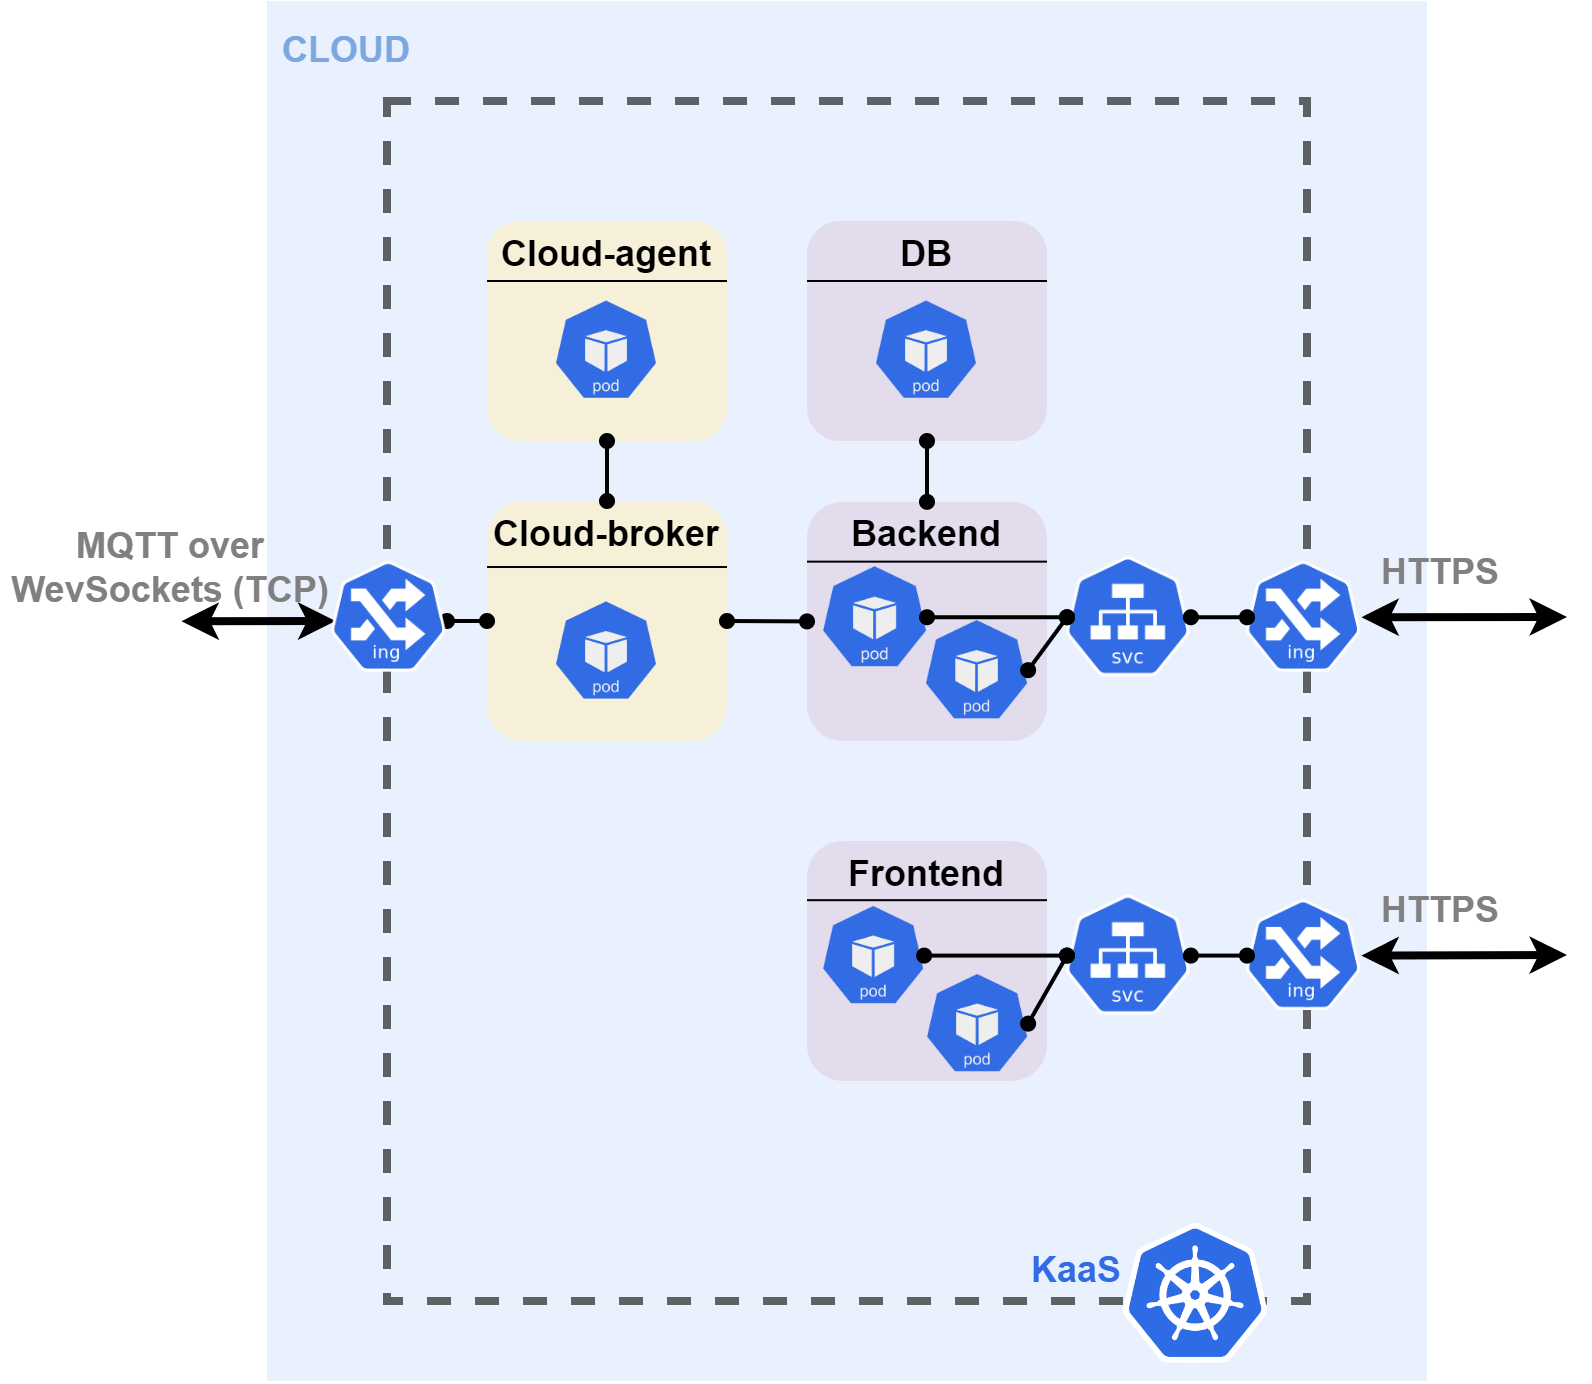
\includegraphics[width=0.8\textwidth]{pictures/cloud_services.png}
    \caption{ Cloud services system design }
    \label{fig:cloud_services}
\end{figure}

Three endpoints are exposed to externally traffic(from outside of the cluster): two HTTP endpoints for Backend and Frontend and one MQTT enpoint for cloud-broker.
HTTP traffic is being served via ingress resources in the cluster it is forwarded via reverse proxy to kubernetes service which distributes the request among the pods. Default ingress resource is designed to only serve HTTP/HTTPS request and do not allow any other protocol. For MQTT protocol which is transported over TCP NodePort is used to expose service to outside world and map pod ports to ports of the node in a cluster.